\begin{figure}[H]
		\begin{minipage}[t]{0.45\linewidth}
		\centering
		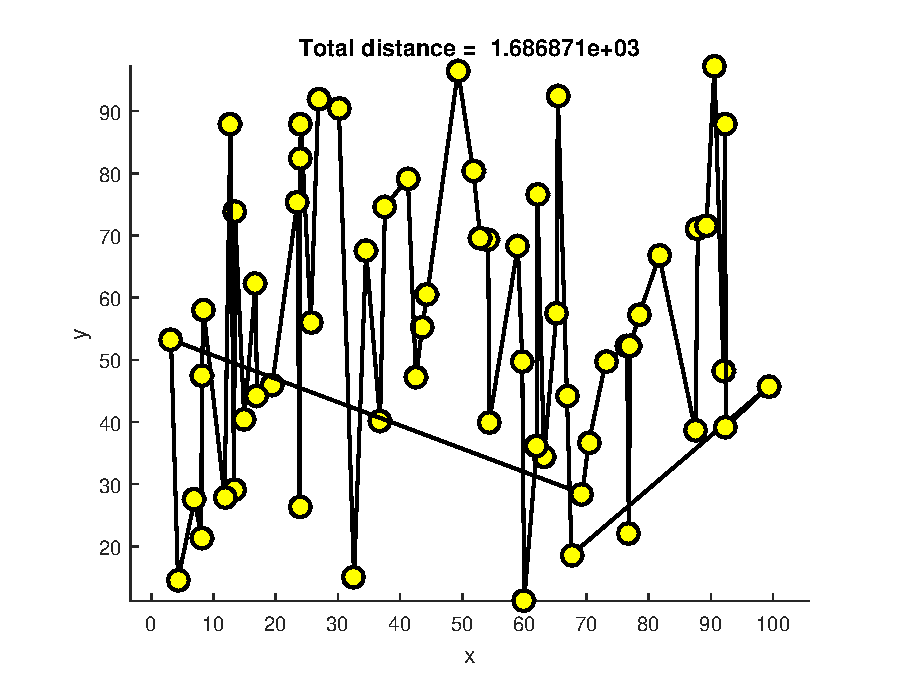
\includegraphics[width=\textwidth]{\Pathofhuit/path.eps}
		\caption{Path journey}\label{fig:Pathofhuit:path}
		
		\end{minipage}\hfill
		\begin{minipage}[t]{0.45\linewidth}
		\centering
		\includegraphics[width=\textwidth]{\Pathofhuit/AS_1_5AS_ExecTimeAndMeanSTDWith_execVariation.eps}
		\caption{Variation of the execution time VS the \# of ants (20$\stackrel{step=20}{\rightarrow}$100) in each execution (1$\stackrel{step=1}{\rightarrow}$ 5)}
		\label{fig:Pathofhuit:AS_1_5AS_ExecTimeAndMeanSTDWith_execVariation}
		\end{minipage}
	\flushleft
		\begin{minipage}[t]{0.45\linewidth}
		\centering
		\includegraphics[width=1.5\textwidth]{\Pathofhuit/AS_BestCost_Varying_Iteration_and_nbAnts.eps}
		\caption{Best cost VS Ants number variation with $\alpha$=1, $ \beta $ = 5}
		\label{fig:Pathofhuit:AS_BestCost_Varying_Iteration_and_nbAnts}
		\end{minipage}
	\end{figure}\flushright
		\begin{minipage}[t]{0.9\linewidth}
		\vspace{-9mm}
		\begin{table}[H]
		\label{tab:Pathofhuit:expdeux}
		\begin{tabular}{lllll}
		\cline{1-2}
		\multicolumn{1}{|l|}{Best Costs results for experience 2}                                                           &  \multicolumn{1}{l|}{Elapsed Time, Mean, STD}                                             &  &  &  \\ \cline{1-2}
		\multicolumn{1}{|l|}{\begin{tiny}\begin{tabular}{|l|c|c|c|c|c|c|c|c|c|c|}
\hline
&\textbf{It :1}&\textbf{It :2}&\textbf{It :3}&\textbf{It :4}&\textbf{It :5}&\textbf{It :6}&\textbf{It :7}&\textbf{It :8}&\textbf{It :9}&\textbf{It :10}\\\hline
\textbf{exec :1}&899.22&899.22&899.22&876.49&876.49&876.49&876.49&876.49&876.49&876.49\\\hline
\textbf{exec :2}&888.19&823.22&823.22&823.22&823.22&823.22&823.22&823.22&823.22&821.34\\\hline
\textbf{exec :3}&890.04&890.04&868.88&868.88&868.88&868.88&868.88&868.88&868.88&868.88\\\hline
\textbf{exec :4}&940.37&867.84&867.84&867.84&867.84&867.84&867.84&867.84&867.84&867.84\\\hline
\textbf{exec :5}&935.28&902.33&902.33&862.38&862.38&862.38&836.13&836.13&836.13&836.13\\\hline
\textbf{exec :6}&854.73&854.73&854.73&854.73&854.73&854.73&854.73&854.73&854.73&854.73\\\hline
\textbf{exec :7}&875.20&875.20&875.20&875.20&875.20&875.20&857.82&857.82&857.82&857.82\\\hline
\textbf{exec :8}&879.70&879.70&879.70&879.70&840.40&840.40&840.40&840.40&840.40&840.40\\\hline
\textbf{exec :9}&902.94&893.72&893.72&893.72&893.72&883.77&883.77&883.77&868.29&849.40\\\hline
\textbf{exec :10}&881.72&821.16&821.16&821.16&821.16&821.16&821.16&821.16&821.16&821.16\\\hline
\end{tabular}
\end{tiny}} & \multicolumn{1}{l|}{\begin{tiny}\begin{tabular}{|l|c|}
\hline
&\textbf{Elapsed time}\\\hline
\textbf{exec :1}&1.94\\\hline
\textbf{exec :2}&3.27\\\hline
\textbf{exec :3}&4.66\\\hline
\textbf{exec :4}&5.97\\\hline
\textbf{exec :5}&7.28\\\hline
\textbf{exec :6}&14.27\\\hline
\textbf{exec :7}&20.91\\\hline
\textbf{exec :8}&27.21\\\hline
\textbf{exec :9}&34.11\\\hline
\textbf{exec :10}&66.83\\\hline
\textbf{ Mean}&18.64\\\hline
\textbf{ STD}&20.17\\\hline
\end{tabular}
\end{tiny} } &  &  &  \\ \cline{1-2}
																						  &                                                                     &  &  &  \\
																						  &                                                                     &  &  & 
		\end{tabular}
		\caption{Results of experience 2 on rand80.dat}
		\end{table}
		\end{minipage}	

%%\end{figure}